\chapter{DI, TPI, y el fenómeno actual que me está sucediendo}

	\noindent
	Ambas, la DI y la TPI, son ``juegos cardinales''. La DI es más vieja y es menos ``rigurosa'' en su exposición. Las dos parten del supuesto, que si el conjunto que hace el papel de Dominio, es ABSURDAMENTE mucho mayor que el otro, si su diferencia cardinal es INCONMENSURABLE, :D, no deberían poder construirse con éxito. Y si se construyen con éxito, ambas implican que el cardinal del Dominio, NO es mayor que el cardinal del otro conjunto (que no tiene por qué ser el conjunto Imagen, ojo). Lo cual implica que pueden ser iguales.

	\section{DI:variante pelea de colegio}
	
	\noindent
	DI significa Diagonalización Inversa. Busca un fenómeno similar a la diagonalización, invirtiendo los papeles conocidos de las cardinalidades $\aleph_{1}$ y $\aleph_{0}$. Da igual que barras todas las opciones disponibles para el Dominio ($\aleph_{1}$), NUNCA podrá 'cubrir´ todos los elementos del conjunto con cardinalidad $\aleph_{0}$.
	\\\\
	
	\noindent
	Consiste en que dos alumnos de un colegio se quieren pelear, comparando la cantidad de amigos que cada uno puede aportar a la pelea. Los amigos de Domenicus (Dominio: D) y los amigos de Luciferio\footnote{Lucifer: portador de Luz, Luz $\rightarrow$ Imagen :D.} (Imagen: I). Domenicus le ha dicho a Luciferio que las paradojas híbridas no existen, y no le deja a Luciferio reproducir el experimento que así lo demuestra\footnote{Déjame descargar frustración en alguna parte...}. Antes de que esta afrenta al honor acabe en un baño de sangre, Luciferio le dice a Domenicus que más le vale rendirse ya que tiene amigos suficientes como para estar en una proporción 2 a 1 o superior.
	\\\\
	
	\noindent
	Domenicus no se fía de Luciferio, tiene fama de tramposo, así que le exige una lista detallada que diga, exactamente, que amigos suyos se van a pelear con cada uno de sus amigos. Así que Luciferio le entrega este esquema (Empecemos por un caso finito, para entender el juego):
	\\\\
	
	\noindent
	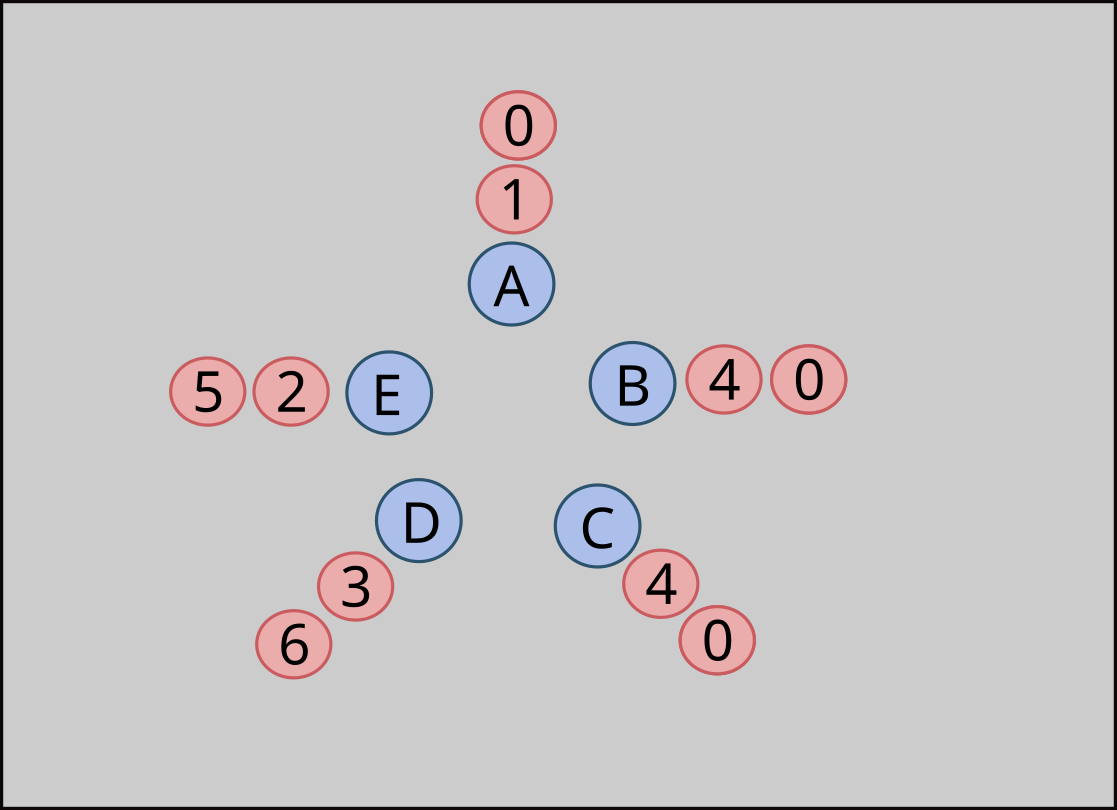
\includegraphics[scale=0.5]{Distribucion_001_A}\\\\
	Como en este colegio son gente muy rara, los amigos de Domenicus tienen nombre de letra, y los de Luciferio tienen nombre de número natural. Vemos que cada amigo de Domenicus(D) tiene un ``Pack'' de amigos de Luciferio(I) asignados. El cardinal de esos Packs es de 2... así que aparentemente Luciferio no mentía con su amenaza.
	\\\\
	
	\noindent
	Después de observar un rato, Domenicus se da cuenta que Luciferio ha hecho trampas: ha puesto a su amigo ``$0$'', dentro del Pack de dos de sus amigos: A y B. Se queja a Luciferio, y este le dice: ``¿Sabes qué, quita a $0$ de la pelea, lo retiro, y si encuentras más repeticiones de uso, también los retiraré de la pelea''. Domenicus luego se fija en que $0$ también está dentro del Pack de C. Luciferio le dice que cuando apartas a uno de sus amigos de la pelea, eso significa quitarlo de TODOS los Packs donde pudiese estar. Así lo hacen y el esquema queda así:\\\\
	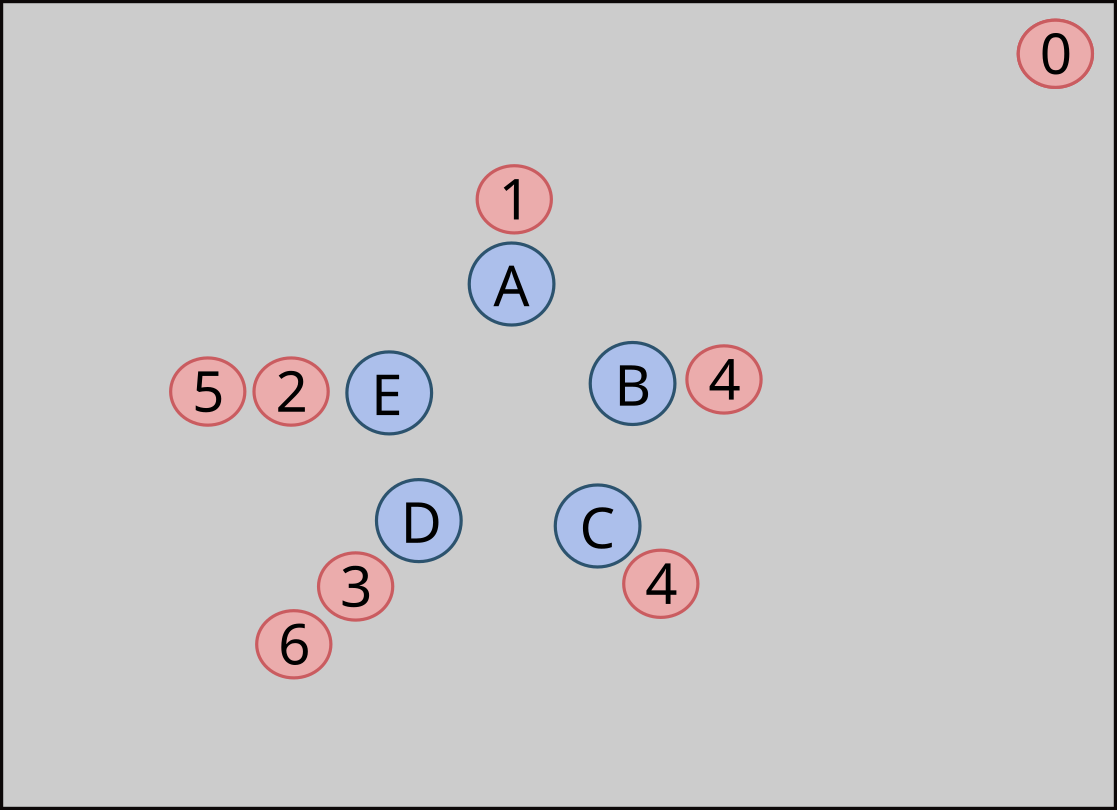
\includegraphics[scale=0.5]{Distribucion_001_B}
	\\\\
	
	\noindent
	Domenicus, que es conocedor de técnicas secretas y avanzadas en teoría de conjuntos, sigue buscando par por par, para ver si Luciferio ha hecho más trampas o si efectivamente, después de descartar a $0$, los Packs nuevos creados a partir del primer esquema (la relación no aplicación original), cumplen las condiciones del Naive CA Theorem.
	\\\\
	
	\noindent
	Domenicus pregunta por el actual estado de los D-pares (E,D), (D,C), (E,A)... (A,B). Los nuevos Packs de (A,B) son más pequeños que los originales, pero ahora son disjuntos, así que este D-par no da más problemas. Y cuando se empieza a desesperar, Domenicus encuentra el D-par (B,C). Tienen el 4 repetido. Siguiendo el acuerdo con Luciferio, 4 se retira de la pelea y lo ``retiran'' de todos los Packs donde pudiese estar:
	\\\\
	
	\noindent
	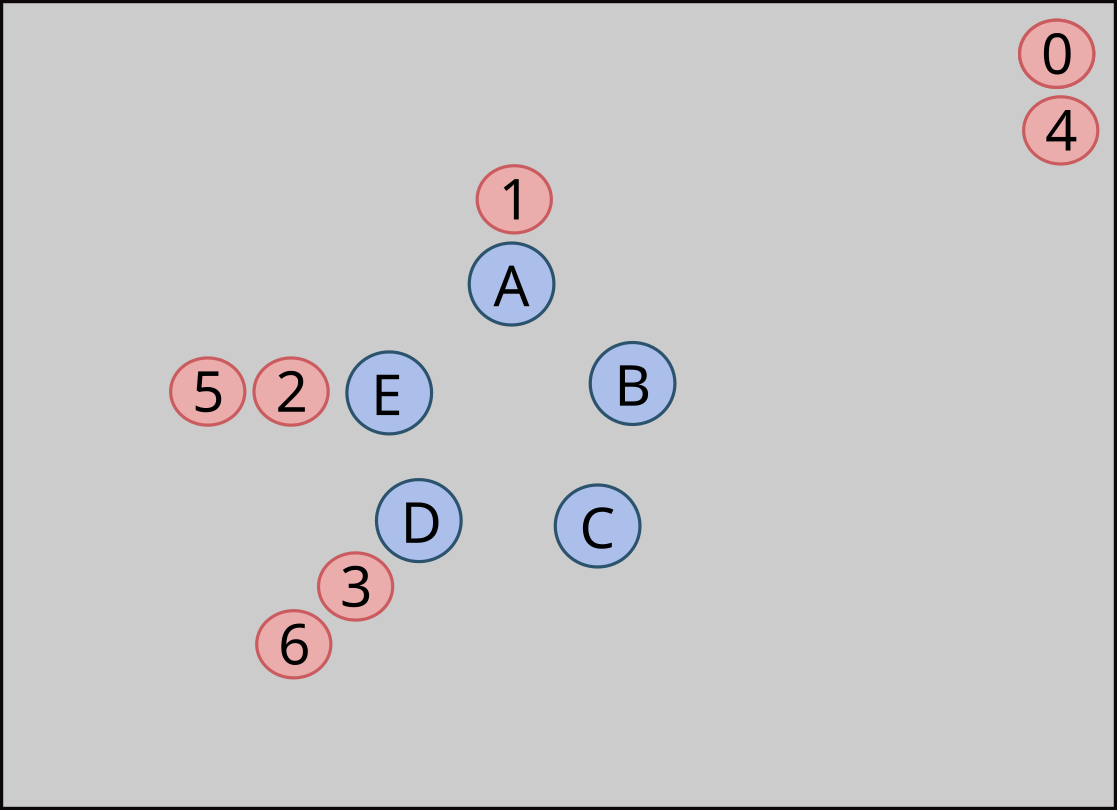
\includegraphics[scale=0.45]{Distribucion_001_C}
	\\\\
	
	\noindent
	Ahora, B y C, tienen Packs asignados completamente vacíos. Domenicus se ríe de Luciferio:``No solo mentiste con la proporción 2 a 1, sino que ni siquiera cumples el Naive CA theorem!!''. Luciferio se enfada mucho, llama a más amigos e intenta otra distribución nueva:
	\\\\
	
	\noindent
	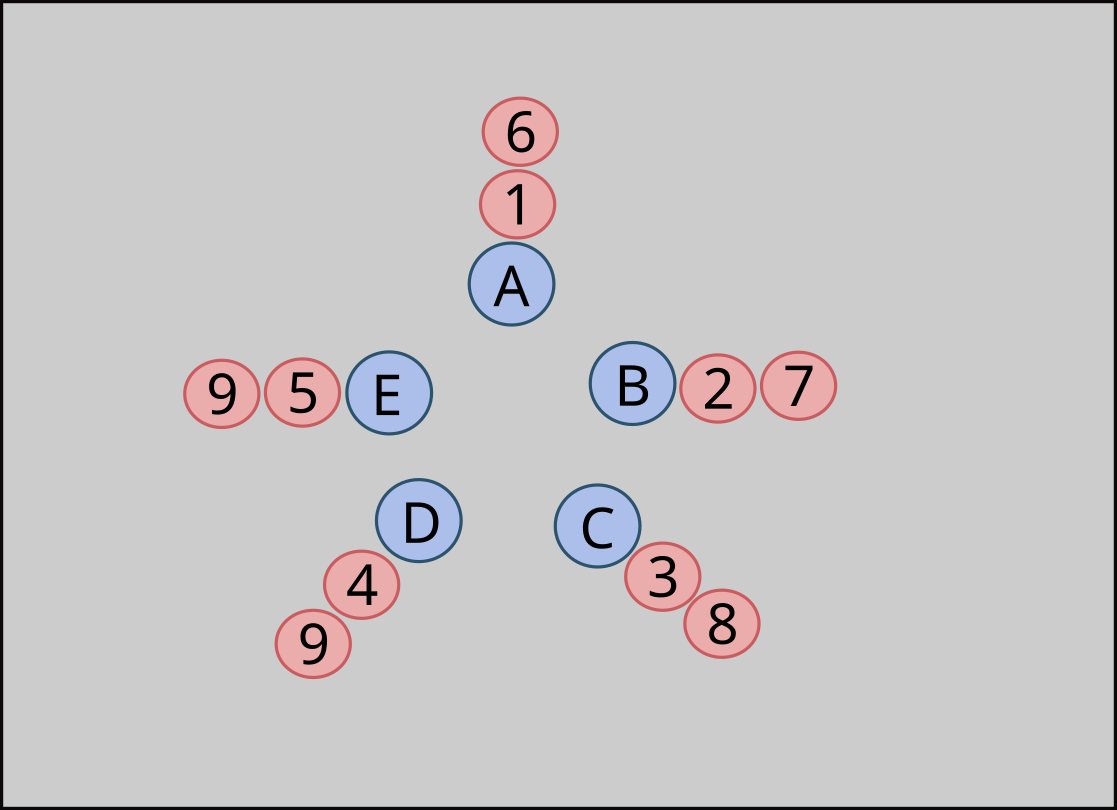
\includegraphics[scale=0.45]{Distribucion_002_A}
	\\\\
	
	\newpage
	

	\noindent
	Rápidamente Domenicus se fija en el D-par (E, D) que repiten el uso del colega 9. Lo apartan y los Packs quedan así:\\\\
	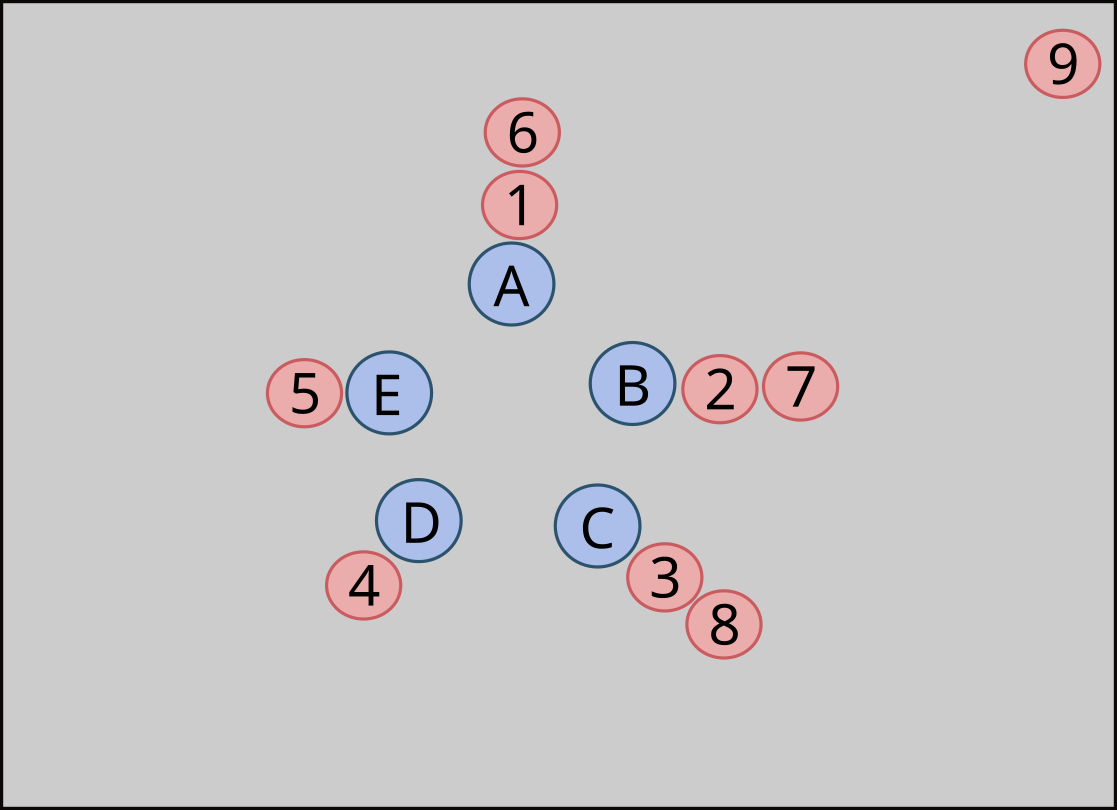
\includegraphics[scale=0.45]{Distribucion_002_B}
	\\\\
	
	\noindent
	Después de este movimiento, Domenicus busca con desesperación otros D-pares con Packs que no sean disjuntos pero ya no encuentra ninguno. La nueva distribución cumple las condiciones del Naive Ca Theorem. Luciferio no cumplió su amenaza totalmente de conseguir una proporción 2 a 1, pero donde no le iguala en número, le supera. Cumplir las condiciones del Naive Ca Theorem indica igualdad de elementos, o algo peor. Se sabe en inferioridad numérica, y aparte debe confiar en que Luciferio no use a sus amigos `` apartados''. Lo cual empeora la inferioridad numérica.
	
	\subsection{Observaciones de la DI}
	
	\noindent
	Partimos de una relación original, posiblemente que no sea aplicación, que está PREDEFINIDA antes de comenzar el juego y que define un conjunto Imagen para cada elemento del Dominio. A partir de ellos, tratamos de ``escoger'' Packs disjuntos, estables, para conseguir cumplir las condiciones del Naive CA Theorem.
	\\\\
	
	\noindent
	Nuestros Packs, comienzan siendo el conjunto Imagen de cada elemento. Según otra persona cualquiera, va escogiendo elementos aleatorios del conjunto Dominio X Dominio, vamos ``recortando''\footnote{A esto lo llamamos en inglés el proceso de ``chopping''} los Packs, eliminando los elementos, no solo de dentro de ellos, sino de cualquier lugar en el que aparezcan en la relación.
	\\\\
	
	\noindent
	No siempre, al preguntar por un D-par, nos obligará a recortar los Packs. A veces, según el orden por el que se pregunte por los D-pares, al preguntar por un D-par concreto, ya habremos eliminado los elementos que impedían a sus Packs ser disjuntos... así que recortar los Packs depende INCLUSO del orden en que recorramos los D-pares.
	\\\\
	
	\noindent
	Si después de haber preguntado por TODOS los D-pares, ninguno de los Packs es vacío, y tienen al menos, un solo elemento, hemos ganado el juego. Cumplimos las condiciones del Naive Ca Theorem:\\
	1) Hay un Pack por cada elemento del Dominio.\\
	2) Cada Pack es No vacío.\\
	3) Todos los Packs son disjuntos entre sí (pq hemos recorrido todos los D-pares y hemos eliminado los elementos que lo impedían).\\
	PODEMOS afirmar que $|Dominio|\ngtr |Imagen|$.
	\\\\
	
	\noindent
	Nuestro ``conjunto especial'' no es uno, sino varios. Son los conjuntos que nos permiten medir el éxito de nuestra labor de forma objetiva. Son los Packs, actuando y sufriendo el ``chopping'' en paralelo. CONSEGUIMOS construir la DI, si algún elemento sobrevive al proceso de ``chopping''. SI NUESTROS CONJUNTOS NO SE VACÍAN. Solo nos hace falta un único elemento, solo uno, por cada Pack (o más). A la misma vez, da igual el éxito del resto, solo un Pack vacío indicará nuestro fracaso. No podremos afirmar nada con seguridad.
	\\\\
	
	\noindent
	El proceso de chopping, se puede definir como una intersección, por cada Pack. Una intersección diferente por cada Pack. Una intersección entre todos los sub-estados de ese Pack. Si el Pack fuese el conjunto $P$, y sus sub-estados, subconjuntos de $P$ llamados $P_{i}$, se cumpliría:\\
	$P_{i+1} \subset P_{i}$\\
	El siguiente estado, en caso de haber un recorte, es el mismo conjunto anterior, pero al que le hemos quitado algunos elementos.\\
	La intersección para cada Pack sería algo así como:\\
	$P_{0} \cap P_{1} \cap P_{2} \cap P_{3} \cap ... \cap P_{final}= ?$
	\\\\
	
	\noindent
	Como los conjuntos infinitos hacen sus locuras, el ÚNICO punto débil de la DI va a ser la interpretación de dichas intersecciones: ¿Si la intersección da un resultado de vacío podemos afirmar que los Packs se vacían? Y esto que parece una pregunta sencilla aparentemente, hay matemáticos que dicen que aunque el resultado sea vacío, no indica ``siempre'' que los Packs se vacían. Otros dicen que ES OBVIO, que si la intersección tiene un resultado INNEGABLE de vacío, indica que los Packs se han vaciado.
	\\\\
	
	\noindent
	La intersección es necesaria porque un proceso secuencial infinito de chopping, NO TIENE FIN... no hay un $P_{final}$. Pero una intersección puede tener términos infinitos, que yo sepa, si estos tienen un cardinal $\aleph_{0}$. Así que nos podemos preguntar por su resultado, y tratar de interpretarlo.
	\\\\
	
	\noindent
	En el futuro de este documento y otros, veremos que el resultado de vacío es inamovible para la flja\_abstracta en el caso $P(\mathbb{N})$ vs $\mathbb{N}$:\\
	a) Si escogemos la interpretación de que los Packs se vacían, El Teorema de Cantor sobrevivirá: nuestros Packs no han conseguido que algunos elementos sobrevivan dentro de ellos, al finalizar el proceso de chopping.\\
	b) NO PODEMOS escoger la opción de que no se vacían en este tipo de intersecciones... sin destruir el Teorema de Cantor. Eso significaría que nuestros Packs sobreviven, y se cumple el Naive CA Theorem. Recordemos que en la flja\_abstracta, $P(\mathbb{N})$ es el Dominio, y $\mathbb{N}$ es el conjunto Imagen.
	\\\\
	
	\noindent
	\textit{En realidad el proceso de chopping, es mucho más bestia, vamos a apartar cantidades OBSCENAS.. pero no de números naturales, sino de miembros de $LCF_{2p}$, el equivalente transformado de $\mathbb(N)$, y el otro conjunto será SNEIs, que será el equivalente transformado de $P(\mathbb{N})$, pero explicar eso requiere más tiempo y contexto.}
	\\\\
	
	\newpage
	
	\section{TPI}
	
	\noindent
	TPI significa Transferencia de Pares Ilimitada... pero ¿Entre qué?¿Qué pares?
	
	\subsection{Definicones previas para entender la TPI}
	\noindent
	Sea $A=\{0,1,2,3,4,5,6,7,8,9\}$\\\\
	Sea $B_{1} = \{a\}$\\\\
	Si intentásemos crear una relación inyectiva entre ambos, usando $A$ como conjunto Dominio y $B_{1}$ como conjunto Imagen, sería completamente imposible. Pero intentemos definir una posible candidata para explicar las medidas que vamos a presentar. \textbf{TODOS los elementos del Dominio deben tener imagen para que tengan sentido}. Los pares de la relación, los definiremos mediante elementos de cada conjunto unidos por flechas:\\\\
	Llamemos a esta relación $r_{1}$
	\begin{table}[h!]
		\begin{tabular}{|c|c|c|c|c|}
			\hline
			$0 \longrightarrow a$ & $1 \longrightarrow a$ & $2 \longrightarrow a$ & $3 \longrightarrow a$ & $4 \longrightarrow a$ \\ 
			\hline
			$5 \longrightarrow a$ & $6 \longrightarrow a$ & $7 \longrightarrow a$ & $8 \longrightarrow a$ & $9 \longrightarrow a$ \\  
			\hline
		\end{tabular}
	\end{table}
	
	\noindent
	Nos podríamos preguntar cuántos pares de $A X A$, cumplen la definición de inyectividad en esa relación concreta. Cuántos RESUELVE ésta relación. ``Resolver'' es un concepto que ya conocemos.\\\\
	$WSP(r_{1})$: $<$Well Solved Pairs$>$ es el subconjunto de elementos de $A X A$, que cumplen la definición de inyectividad, en ESA relación.\\\\
	$NWSP(r_{1})$: $<$NOT Well Solved Pairs$>$ es el subconjunto de elementos de $A X A$, que \textbf{NO} cumplen la definición de inyectividad, en ESA relación.\\\\
	Ambos conjuntos son complementarios respecto de $A X A$. WSP es el complementario de NWSP y viceversa. El mismo par, no puede estar en WSP y NWSP en la misma relación. O cumple la definición o no la cumple.\\\\
	$QRE(r_{1})$: $<$Quantity of Repeated Elements$>$ es el cardinal de NWSP, en ESA relación.
	\\
	
	\noindent
	A pesar de que la relación que hemos creado, es uno de los posibles ejemplos más desastrosos que pueden haber, la definición de inyectividad nos permite dar por válidos aquellos pares que están formados por el mismo elemento del Dominio. En esos casos, da igual que tengan la misma imagen en la relación, son pares correctos. Van en WSP.
	\\
	
	\noindent
	$WSP(r_{1}) = \{(0,0), (1,1), (2,2), ..., (8,8), (9,9)\}$\\\\
	En NWSP iría el resto de posibles pares. Entonces:\\\\
	$|WSP_{r_{1}}| = 10$\\\\
	$|NWSP_{r_{1}}| = 90$\\
	*ya que el cardinal de $A X A$ sería 100.\\\\
	$QRE_{r_{1}} = 90$
	\\
	
	\noindent
	Les ponemos un sub-indicativo, porque no solo dependen de los conjuntos involucrados, sino de la relación que hemos decidido crear entre ellos.
	\\
	
	\noindent
	Cuando $QRE=0$, significa que el cardinal de NWSP es cero. Eso implica que es un conjunto vacío. O sea, que NO EXISTEN pares que INCUMPLAN la definición de inyectividad. Cuando $QRE=0$, o $NWSP=\emptyset$, indica que es una relación inyectiva, perfecta.
	\\
	
	\newpage
	\section{$r_{2}$: 10 vs 2}
	
	\noindent
	Sea $A=\{0,1,2,3,4,5,6,7,8,9\}$\\\\
	Sea $B_{2} = \{a,b\}$
	\\
	
	\noindent
	$r_{2a}:A \longrightarrow B_{2}$
	\begin{table}[h!]
		\begin{tabular}{|c|c|c|c|c|}
			\hline
			$0 \longrightarrow b$ & $1 \longrightarrow b$ & $2 \longrightarrow b$ & $3 \longrightarrow b$ & $4 \longrightarrow b$ \\ 
			\hline
			$5 \longrightarrow b$ & $6 \longrightarrow b$ & $7 \longrightarrow b$ & $8 \longrightarrow b$ & $9 \longrightarrow b$ \\  
			\hline
		\end{tabular}
	\end{table}
	
	\noindent
	En esta relación hemos optado por ni siquiera usar todos los elementos del conjunto Imagen. Un auténtico desastre. Pero un desastre muy parecido al ejemplo de relación del punto anterior: $r_{1}$. Es idéntica solo que cambiando la `a' por la `b'. Las medidas son iguales:\\
	$|WSP_{r_{2a}}| = 10$\\
	$|NWSP_{r_{2a}}| = 90$\\
	$QRE_{r_{2a}}=90$
	\\
	
	\noindent
	$r_{2b}:A \longrightarrow B_{2}$
	\begin{table}[h!]
		\begin{tabular}{|c|c|c|c|c|}
			\hline
			$0 \longrightarrow a$ & $1 \longrightarrow b$ & $2 \longrightarrow b$ & $3 \longrightarrow b$ & $4 \longrightarrow b$ \\ 
			\hline
			$5 \longrightarrow b$ & $6 \longrightarrow b$ & $7 \longrightarrow b$ & $8 \longrightarrow b$ & $9 \longrightarrow b$ \\  
			\hline
		\end{tabular}
	\end{table}
	
	\noindent
	En este ejemplo ya hemos usado los dos elementos del conjunto Imagen, pero no nos hemos esforzado demasiado. Aún así, las medidas mejoran. Antes, el par $(0,1)$ estaba en NWSP, y ahora está en WSP. Aparte de los 10 pares, que están formados por el mismo elemento, a WSP llegan los pares que contengan el 0, pues este está relacionado con un elemento único del conjunto Imagen. Nadie más esta relacionado con `a', solo el 0. A la hora de contar, conviene recordar que en $A X A$, los pares $(0,1)$ y $(1,0)$, por ejemplo, no son el mismo, aunque sepamos seguro que si uno cumple la definición de inyectividad, el otro también. En general, resolver el par $(i,j)$ es lo mismo que resolver el par $(j,i)$. Las medidas quedan:\\
	$|WSP_{r_{2b}}| = 10+(9*2) = 28$\\
	$|NWSP_{r_{2b}}| = 72$\\
	$QRE_{r_{2b}}=72$
	\\
	
	\noindent
	$r_{2}:A \longrightarrow B_{2}$
	\begin{table}[h!]
		\begin{tabular}{|c|c|c|c|c|}
			\hline
			$0 \longrightarrow a$ & $1 \longrightarrow a$ & $2 \longrightarrow a$ & $3 \longrightarrow a$ & $4 \longrightarrow a$ \\ 
			\hline
			$5 \longrightarrow b$ & $6 \longrightarrow b$ & $7 \longrightarrow b$ & $8 \longrightarrow b$ & $9 \longrightarrow b$ \\  
			\hline
		\end{tabular}
	\end{table}
	
	\noindent
	Aquí si me he esforzado más. No estoy seguro de que sea la mejor relación posible. Al crear esta, sabemos que, al menos, estas medidas son posibles:\\
	$|WSP_{r_{2}}| = 10+(5*5*2) = 60$\\
	$|NWSP_{r_{2}}| = 40$\\
	$QRE_{r_{2}}=40$
	\\
	
	
	\noindent
	Me gusta decir que QRE es una medida inestable, pero de tipo `record del mundo': no se sabe si alguien la puede mejorar, pero una vez existe una, sabemos seguro que ese valor es posible. Y si con las relaciones que obtengamos, conseguimos resultados `suficientes' para nuestros objetivos, que alguien más pueda encontrar otra relación con mejores medidas nos va a dar igual. Ya encontramos lo que necesitábamos. Para salvarte de un zombie no necesitas ser el corredor más rápido del mundo, solo ser más rápido que el más lento de tu grupo.
	\\
	
	\noindent
	También podemos observar, como al tener más elementos disponibles en el conjunto Imagen, tenemos `potencial' para mejorar las medidas. No es seguro que lo logremos. Depende de nuestra capacidad para crear las relaciones. Podemos usar muy mal los elementos del conjunto imagen, o muy bien. 
	\\
	
	\noindent
	Se intuye que debe existir un tope, a la cantidad de pares que podemos incluir en WSP, cuando el conjunto Imagen tiene un cardinal inferior, estrictamente, al del conjunto Dominio. Como es el caso aquí:\\ 
	$|B_{2}|=2$\\ 
	$|A|=10$\\
	Por muy bien que lo hagamos, conseguir un QRE=0 para una relación del tipo\\
	$r:A \longrightarrow B_{2}$\\
	sería un absurdo!! Al mismo tiempo, que ese `tope' no exista, sería un posible indicativo de que nos hemos equivocado al juzgar el cardinal del conjunto Imagen, por la causa que sea.
	\\
	
	\noindent
	También, como empezamos a decir dos párrafos más arriba, cuántos más elementos tenemos en nuestro conjunto Imagen, más fácil nos resulta hacer más chiquitito a NWSP. Ya definiremos que consideramos una mejora. En los ejemplos de cardinalidad finita es muy fácil verlo. La medida QRE habla por sí sola. En los conjuntos de cardinalidad infinita no tanto.
	\\
	
	\newpage
	\section{$r_{3}$: 10 vs 5}
	
	\noindent
	Sea $A=\{0,1,2,3,4,5,6,7,8,9\}$\\\\
	Sea $B_{3} = \{a,b,c,d,e\}$
	\\
	
	\noindent
	Sea $r_{3}:A \longrightarrow B_{3}$
	\begin{table}[h!]
		\begin{tabular}{|c|c|c|c|c|}
			\hline
			$0 \longrightarrow a$ & $1 \longrightarrow b$ & $2 \longrightarrow c$ & $3 \longrightarrow d$ & $4 \longrightarrow e$ \\ 
			\hline
			$5 \longrightarrow a$ & $6 \longrightarrow b$ & $7 \longrightarrow c$ & $8 \longrightarrow d$ & $9 \longrightarrow e$ \\  
			\hline
		\end{tabular}
	\end{table}
	
	\noindent
	Ahora resulta más fácil ver que pares caen en $NWSP$: \\\\
	$NWSP_{r_{3}}=\{ (0,5), (5,0), (1,6), (6,1), (2,7), (7,2), (3,8), (8,3), (4,9), (9,4)\}$\\
	$|NWSP_{r_{3}}| = 10$\\
	Esto implica que, como son complementarios:\\
	$|WSP_{r_{3}}| = 90$\\
	$QRE_{r_{3}}=10$
	\\
	
	\section{$r_{4}$: 10 vs 9}
	
	\noindent
	Sea $A=\{0,1,2,3,4,5,6,7,8,9\}$\\\\
	Sea $B_{4} = \{a,b,c,d,e,f,g,h,i\}$
	\\
	
	\noindent
	Sea $r_{4}:A \longrightarrow B_{4}$
	\begin{table}[h!]
		\begin{tabular}{|c|c|c|c|c|}
			\hline
			$0 \longrightarrow a$ & $1 \longrightarrow b$ & $2 \longrightarrow c$ & $3 \longrightarrow d$ & $4 \longrightarrow e$ \\ 
			\hline
			$5 \longrightarrow f$ & $6 \longrightarrow g$ & $7 \longrightarrow h$ & $8 \longrightarrow i$ & $9 \longrightarrow e$ \\  
			\hline
		\end{tabular}
	\end{table}
	
	\noindent
	Ahora solo hay dos pares que caen dentro de $NWSP$: \\\\
	$NWSP_{r_{4}}=\{ (4,9), (9,4) \}$\\
	$|NWSP_{r_{4}}| = 2$\\
	$|WSP_{r_{4}}| = 98$\\
	$QRE_{r_{4}}=2$
	\\
	
	\noindent
	Sabemos que es el mejor caso posible, porque un $QRE=0$ es imposible. Y no puedes resolver $(4,9)$ sin resolver $(9,4)$.
	\\
	
	\noindent
	Observemos como según teníamos más elementos disponibles, nuestro valores QRE se acercaban a cero:\\
	$ |B_{1}| = 1 \:\:\:\:\:\:\:\:\: \rightarrowtail \:\:\:\:\:\:\:\:\: QRE_{r_{1}} = 90$\\
	$ |B_{2}| = 2 \:\:\:\:\:\:\:\:\: \rightarrowtail \:\:\:\:\:\:\:\:\: QRE_{r_{2}} = 40$\\
	$ |B_{3}| = 5 \:\:\:\:\:\:\:\:\: \rightarrowtail \:\:\:\:\:\:\:\:\: QRE_{r_{3}} = 10$\\
	$ |B_{4}| = 9 \:\:\:\:\:\:\:\:\: \rightarrowtail \:\:\:\:\:\:\:\:\: QRE_{r_{4}} = 2$\\
	
	\newpage
	
	
	
	\section{Resultado increíble}